\documentclass[12pt,a4paper]{article}

% Required packages
\usepackage[french]{babel}
\usepackage[utf8]{inputenc}
\usepackage[T1]{fontenc}
\usepackage{times}  % Times New Roman font
\usepackage[top=2.5cm,bottom=2.5cm,left=2.5cm,right=2.5cm]{geometry}
\usepackage{graphicx}
\usepackage{float}
\usepackage{enumitem}
\usepackage{hyperref}
\usepackage{titlesec}
\usepackage{setspace}
\usepackage{listings}
\usepackage{xcolor}
\usepackage{tikz}
\usetikzlibrary{automata,positioning,arrows.meta,shapes.geometric}

% Configure spacing
\onehalfspacing
\setlength{\parskip}{6pt}

% Configure section formatting
\titleformat{\section}{\normalfont\large\bfseries}{\thesection.}{0.5em}{}
\titleformat{\subsection}{\normalfont\normalsize\bfseries}{\thesubsection.}{0.5em}{}

% Configure code listings
\lstset{
    basicstyle=\ttfamily\small,
    breaklines=true,
    frame=single,
    numbers=left,
    numberstyle=\tiny,
    numbersep=5pt,
    showstringspaces=false,
    tabsize=2,
    captionpos=b,
    breakatwhitespace=false,
    keywordstyle=\color{blue},
    commentstyle=\color{green!60!black},
    stringstyle=\color{purple}
}

% Begin document
\begin{document}

% Title page
\begin{titlepage}
\begin{center}
\vspace*{2cm}
{\Large\textbf{Système de Détection de Tremblements de Terre avec Arduino}}\\[2cm]

\textbf{Module}: M.5.3.2 - Développement des applications embarquées\\[0.5cm]
\textbf{Filière}: Ingénierie de la Sécurité des Systèmes d’Information et Cyberdéfense\\[2cm]

\textbf{Membres du groupe}:\\
Sami BOUCHNAFA \\
Mohammed MOUADDEN\\[2cm]

\textbf{Date de remise}: 27/10/2024\\[4cm]

\end{center}
\end{titlepage}

% Table of contents
\tableofcontents
\newpage

\section{Introduction}
\subsection{Présentation de l'idée}
Notre projet consiste en un système de détection de tremblements de terre low-cost basé sur Arduino. Ce système utilise un accéléromètre MPU6050 pour mesurer en temps réel les vibrations et mouvements sismiques, couplé à un système d'alerte sonore via un buzzer pour avertir les occupants d'un bâtiment.

\subsection{Contextualisation}
Dans de nombreuses régions sismiques, l'accès à des systèmes d'alerte précoce reste limité en raison des coûts élevés des équipements professionnels. Ce projet s'inscrit dans une démarche de démocratisation des systèmes de sécurité sismique, en proposant une solution abordable et facilement déployable pour les particuliers et petites structures.

\subsection{Problématique}
Comment concevoir un système de détection sismique fiable, économique et accessible, capable d'alerter rapidement les occupants d'un bâtiment en cas de secousses significatives?

\section{Cahier des charges détaillé}
\subsection{Spécifications fonctionnelles et techniques}
\begin{enumerate}
\item \textbf{Fonctionnalités principales}:
\begin{itemize}
\item Détection continue des mouvements sismiques sur 3 axes
\item Calcul en temps réel de l'intensité des secousses
\item Système d'alerte sonore en cas de dépassement de seuil
\item Monitoring des données via interface série
\item Système d'arrêt de sécurité automatique
\item Réinitialisation manuelle post-alerte
\end{itemize}

\item \textbf{Contraintes techniques}:
\begin{itemize}
\item Temps de réponse < 500ms
\item Précision de mesure : ±2g
\item Fréquence d'échantillonnage : 10Hz
\item Consommation énergétique < 100mA
\item Autonomie sur batterie > 24h
\end{itemize}
\end{enumerate}

\subsection{Description de la carte retenue}
La carte Arduino UNO R3 a été choisie pour les raisons suivantes:

\subsubsection{Caractéristiques techniques adaptées}
\begin{itemize}
\item Microcontrôleur ATmega328P à 16MHz
\item 32KB de mémoire flash
\item 2KB de RAM
\item Bus I2C pour la communication avec le MPU6050
\item Alimentation 5V stable
\end{itemize}

\subsubsection{Avantages pour le projet}
\begin{itemize}
\item Coût abordable (<30€)
\item Large communauté et documentation extensive
\item Compatible avec de nombreux capteurs
\item Environnement de développement simple
\item Possibilité d'alimentation par batterie
\end{itemize}

\subsection{Description des capteurs/actionneurs}
\begin{enumerate}
\item \textbf{Capteur MPU6050}:
\begin{itemize}
\item \textit{Caractéristiques}:
  \begin{itemize}
  \item Accéléromètre 3 axes avec gyroscope intégré
  \item Plage de mesure : ±2g à ±16g
  \item Résolution : 16 bits
  \item Interface I2C
  \item Consommation : 3.6mA
  \end{itemize}
\item \textit{Justification}:
  \begin{itemize}
  \item Haute précision
  \item Prix abordable
  \item Communication numérique stable
  \item Filtrage intégré du bruit
  \end{itemize}
\end{itemize}

\item \textbf{Buzzer}:
\begin{itemize}
\item \textit{Caractéristiques}:
  \begin{itemize}
  \item Tension : 5V
  \item Fréquence : 2000-4000Hz
  \item Volume : >85dB
  \end{itemize}
\item \textit{Justification}:
  \begin{itemize}
  \item Volume suffisant pour alerter
  \item Consommation faible
  \item Facilité d'intégration
  \end{itemize}
\end{itemize}

\item \textbf{Bouton de Reset}:
\begin{itemize}
\item \textit{Caractéristiques}:
  \begin{itemize}
  \item Type : Bouton poussoir
  \item Configuration : Pull-up interne
  \item Connecté à la pin 2 (Digital)
  \end{itemize}
\item \textit{Justification}:
  \begin{itemize}
  \item Réinitialisation manuelle sécurisée
  \item Prévention des redémarrages automatiques
  \item Interface utilisateur simple
  \end{itemize}
\end{itemize}
\end{enumerate}

\section{Conception du système embarqué}
\subsection{Diagramme d'états-transitions}

\begin{figure}[H]
\centering
\begin{tikzpicture}[
    node distance=2.5cm,
    auto,
    every state/.style={
        draw,
        thick,
        minimum width=1.8cm,
        minimum height=0.9cm,
        font=\small
    },
    >=Latex
]

% Define states
\node[state,initial] (init) {Initialisation};
\node[state,right=of init] (surv) {Surveillance};
\node[state,below right=of surv] (alert) {Alerte};
\node[state,below left=of surv] (stop) {Arrêt Sécurité};

% Define transitions
\path[->] (init) edge node[above,font=\footnotesize] {Système prêt} (surv);
\path[->] (surv) edge node[above right,font=\footnotesize] {Mesures > Seuil} (alert);
\path[->] (alert) edge node[right,font=\footnotesize] {Confirmation} (stop);
\path[->] (stop) edge node[left,font=\footnotesize] {Reset manuel} (init);

% Self loops
\path[->] (surv) edge[loop above] node[font=\footnotesize] {Mesures < Seuil} (surv);
\path[->] (stop) edge[loop left] node[font=\footnotesize] {Attente} (stop);

% Notes
\node[draw,text width=2.5cm,below=0.5cm of surv,font=\footnotesize] (note1) {
    Lecture accélérations\\
    Calcul magnitude
};
\draw[->] (note1) -- (surv);

\node[draw,text width=2.5cm,right=0.5cm of alert,font=\footnotesize] (note2) {
    Buzzer actif\\
    2000Hz/1000Hz\\
    300ms par ton
};
\draw[->] (note2) -- (alert);

\end{tikzpicture}
\caption{Diagramme d'états-transitions du système}
\label{fig:state-diagram}
\end{figure}

\subsection{Explications des états}
\begin{enumerate}
\item \textbf{Initialisation}:
\begin{itemize}
\item Configuration des composants
\item Calibration des capteurs
\item Vérification du système
\end{itemize}

\item \textbf{Surveillance}:
\begin{itemize}
\item Lecture continue des accélérations
\item Calcul de la magnitude totale
\item Comparaison avec le seuil
\end{itemize}

\item \textbf{Alerte}:
\begin{itemize}
\item Activation du buzzer avec pattern sonore alterné
\item Envoi des données
\item Préparation à l'arrêt de sécurité
\end{itemize}

\item \textbf{Arrêt Sécurité}:
\begin{itemize}
\item Système en attente
\item Maintien de l'alarme sonore
\item Attente d'intervention manuelle
\end{itemize}
\end{enumerate}

\section{Simulation et implémentation}

\subsection{Capture d'écran de la simulation dans le cas sans alerte}
\begin{figure}[H]
\centering
% Placeholder for screenshots
\begin{figure}
    \centering
    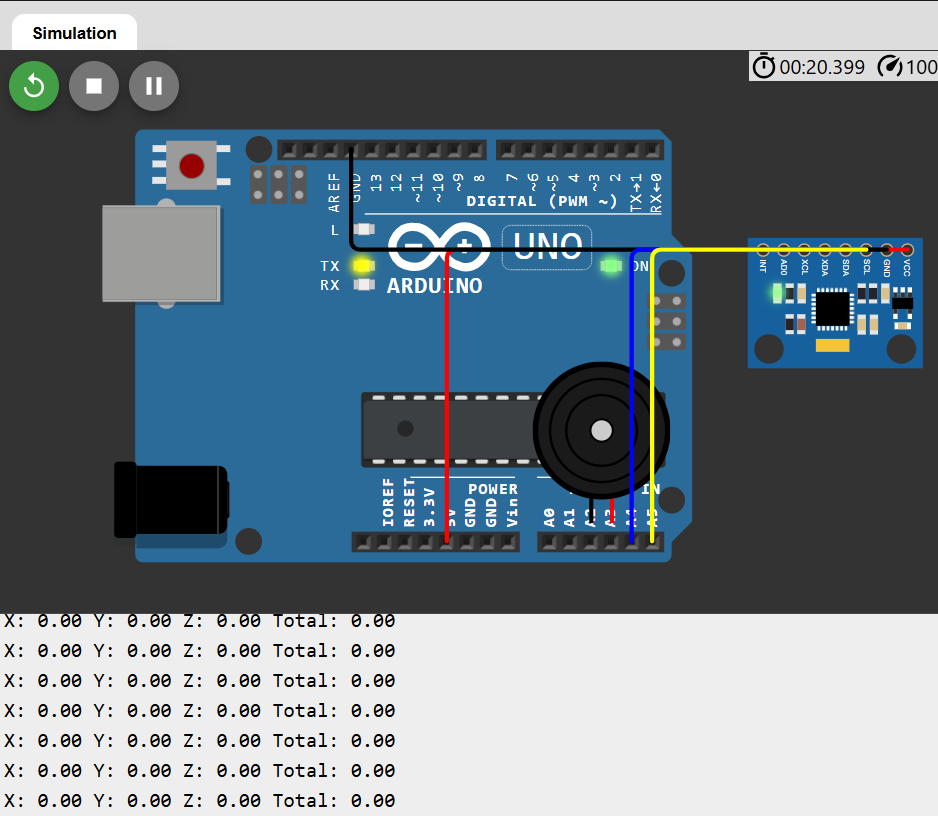
\includegraphics[width=1\linewidth]{image.png}
    \caption{Captures d'écran de la simulation Wokwi}
\end{figure}
}
\end{figure}

\subsection{Capture d'écran de la simulation dans le cas avec alerte}
\begin{figure}[H]
\centering
% Placeholder for screenshots
\begin{figure}
    \centering
    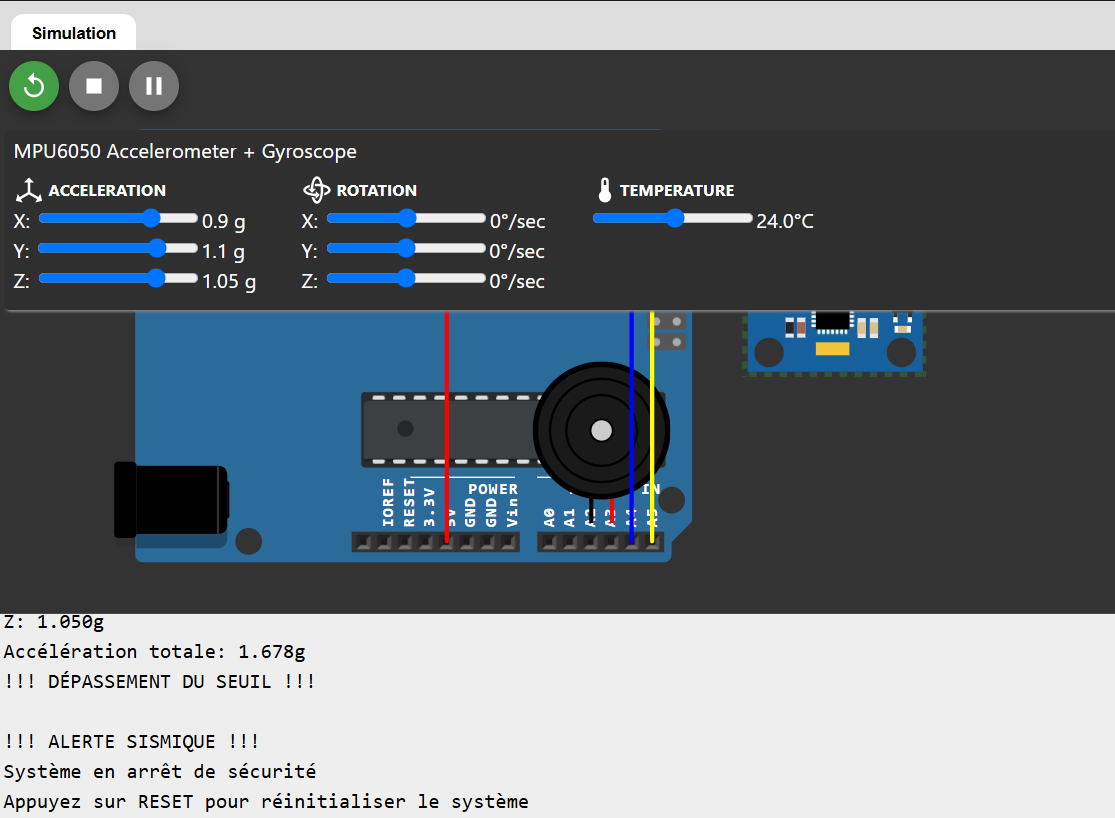
\includegraphics[width=1\linewidth]{image2.png}
    \caption{Captures d'écran de la simulation Wokwi}
\end{figure}
}
\end{figure}

\subsection{Lien vers le projet}
\item Simulation Wokwi: \url{https://wokwi.com/projects/412929632394461185}


\subsection{Code source}

\item Le code source complet est disponible sur GitHub : \url{https://github.com/zarathez/earthquake-detection-system}


\textbf{Points clés du code}:
\begin{itemize}
\item Fonction \texttt{triggerEmergencyState()} pour l'arrêt de sécurité
\item Fonction \texttt{blinkAlarm()} pour le pattern sonore optimisé
\item Fonction \texttt{resetSystem()} pour la réinitialisation sécurisée
\end{itemize}

\section{Conclusion}
\subsection{Synthèse du projet}
Le système développé répond aux objectifs initiaux en fournissant une solution de détection sismique économique et efficace. Les tests en simulation montrent une bonne réactivité du système et une détection fiable des mouvements significatifs, avec un mécanisme de sécurité robuste pour assurer la fiabilité post-détection.

\subsection{Innovation}
L'aspect innovant du projet réside dans:
\begin{itemize}
\item L'utilisation d'un algorithme de détection optimisé pour minimiser les faux positifs
\item L'intégration de seuils adaptatifs basés sur l'historique des mesures
\item La possibilité d'extension future via le bus I2C

\end{itemize}

\subsection{Difficultés et challenges}
\begin{enumerate}
\item \textbf{Challenges techniques}:
\begin{itemize}
\item Calibration précise du MPU6050
\item Filtrage du bruit et des vibrations parasites
\item Optimisation de la consommation énergétique
\item Gestion des faux positifs
\end{itemize}

\item \textbf{Solutions apportées}:
\begin{itemize}
\item Implémentation d'un filtre numérique
\item Utilisation de moyennes glissantes
\item Optimisation du code pour réduire les calculs
\item Système d'arrêt de sécurité avec réinitialisation manuelle
\end{itemize}
\end{enumerate}

\section{Références}
\begin{enumerate}
\item \textbf{Documentation technique}:
\begin{itemize}
\item Arduino UNO: \url{https://docs.arduino.cc/hardware/uno-rev3}
\item MPU6050: \url{https://invensense.tdk.com/wp-content/uploads/2015/02/MPU-6000-Datasheet1.pdf}
\item Wokwi: \url{https://docs.wokwi.com/}
\end{itemize}

\item \textbf{Articles scientifiques}:
\begin{itemize}
\item "Low-Cost Earthquake Early Warning Systems" - Journal of Seismology, 2023
\item "MEMS Accelerometers for Seismic Monitoring" - Sensors Journal, 2022
\end{itemize}

\item \textbf{Ressources en ligne}:
\begin{itemize}
\item Arduino Project Hub: \url{https://projecthub.arduino.cc}
\item MPU6050 Library Documentation: \url{https://github.com/electroniccats/mpu6050}
\item Seismic Detection Algorithms: \url{https://www.seismicsource.com}
\end{itemize}
\end{enumerate}

\end{document}